\section{Experiments}

In this section, we will introduce selected LVLMs for evaluation, experiment results and  analysis. 
% LVLMs we selected to evaluate,
% related

\subsection{Large Vision Language Models}

InstructBLIP-7B \cite{dai2023instructblip}, Qwen-VL-Chat \cite{bai2023qwenvl}, LLaVA-v1.5-7B and LLaVA-v1.5-13B \cite{liu2023improved}, mPLUG-Owl-2 \cite{ye2023mplug}, ShareGPT4V-7B and ShareGPT4V-13B \cite{chen2023sharegpt4v} and GPT-4V \cite{openai2023gpt4} are selected in this paper to be evaluated using CogBench.
% Table \ref{tab:lvlms} shows an overview of the design of different LVLMs.
A brief introduction of these models is shown in Appendix \ref{sec:lvlms}.

% We select the following representative LVLMs for evaluation:

% \begin{itemize}
%     \item \textbf{InstructBLIP} \cite{dai2023instructblip} builds upon BLIP-2 \cite{li2023blip}. 
%     % and restructures 26 publicly available datasets into an instructional tuning format and uses 13 held-in datasets for instruction tuning. 
%     It consists of an image encoder, an LLM, and a Query Transformer (Q-Former). 
%     During instruction tuning, only the Q-Former is updated. We use ``blip2-vicuna-instruct'' for testing.
%     \item \textbf{Qwen-VL-Chat} \cite{bai2023qwenvl} is a instruction-tuned VL chatbot based on Qwen-VL. 
%     % Its training process consists of two stages of pre-training and a final stage of instruction fine-tuning. 
%     As for architecture, it consists of a vision encoder, a LLM, and position-aware vision-language adapter. We test ``Qwen-VL-Chat''.
%     \item \textbf{LLaVA v1.5} \citep{liu2023improved} is an upgraded version of LLaVA  \cite{liu2023llava}. 
%     % LLaVA connects a vision encoder and LLM for general-purpose visual and language understanding. 
%     It is instruction-tuned on the language-image instruction-following data generated by language-only GPT-4 \cite{openai2023gpt4}. 
%     By using CLIP-ViT-L-336px with an MLP projection and adding academic-task-oriented VQA data with simple response formatting prompts, LLaVA v1.5 achieves better performance. 
%     ``llava-v1.5-7b'' and ``llava-v1.5-13b'' are tested.
%     \item \textbf{mPLUG-Owl-2} \cite{ye2023mplug} mainly comprises a fundamental vision encoder, a visual abstractor, and a language decoder. 
%     % It also adopts a two-stage training strategy, comprising pre-training and visual instruction tuning. 
%     We test ``mplug-owl2-llama2-7b''. 
%     \item \textbf{ShareGPT4V} \cite{chen2023sharegpt4v} follows the design of LLaVA v1.5.
%     % 1.2 million
%     % ShareGPT4V dataset
%      They incorporate a large-scale resource featuring highly descriptive captions into both the pre-training and supervised fine-tuning phases of ShareGPT4V model.
%     % The model shows remarkable performance across a majority of the multi-modal benchmarks.
%     We test``ShareGPT4V-7B'' and ``ShareGPT4V-13B''.
%     \item \textbf{GPT-4V} \citep{openai2023gpt4} is one of the most powerful LVLMs in the world developed by OpenAI. The version of ``gpt-4-vision-preview'' is tested.
% \end{itemize}


% \begin{table}
%     \centering
%     \small
%     \begin{tabular}{lll}
%     \hline
%     \textbf{Model} & \thead{\textbf{Visual Encoder} } & \thead{\textbf{Language Model}}\\ % \\ \textbf{Accuracy}
%     \hline
%     InstructBLIP-7B  & EVA-CLIP ViT-g & Vicuna-7B \\
%     Qwen-VL-Chat & OpenCLIP ViT-G & Qwen-7B \\
%     LLaVA-v1.5-7B  & CLIP ViT-L & Vicuna-7B \\
%     LLaVA-v1.5-13B & CLIP ViT-L & Vicuna-13B \\
%     mPLUG-Owl-2 & CLIP ViT-L & LLaMA-7B \\
%     % Otter  &  &   \\
%     % CogVLM & 0 & & & & & & & & \\
%     ShareGPT4V-7B & CLIP ViT-L & Vicuna-7B \\
%     ShareGPT4V-13B & CLIP ViT-L & Vicuna-13B \\
%     % Monkey &  &  \\
%     GPT-4V & \multicolumn{1}{c}{--}  & \multicolumn{1}{c}{--} \\
%     \hline
%     \end{tabular}
%     \caption{\label{tab:lvlms}
%     LVLMs evaluated in this paper.
%     }
% \end{table}


% ShareGPT-4V 

\subsection{Results of Description Task}

% As mentioned earlier, we consider both recognition and cognition ability of LVLMs in CogID task.

% For fair comparison, we use the following prompt for LVLMs to generate image description:

We prompt the selected LVLMs with the following instruction to obtain detailed descriptions about images in CogBench.

\textit{Describe this image in detail.}

Then, we evaluate the performance of LVLMs on Description task in terms of both recognition and cognition ability.

As a reference, we also calculated traditional image captioning evaluation metrics by camparing annotated reference description and model-generated description, and details are shown in Appendix \ref{sec:cap_eval}.

\subsubsection{Recognition}

Table \ref{tab:rec_score} shows the Recognition Score of models on Description task.
GPT-4V achieves the best performance in terms of recognition, which means it can recognize and describe more entities.
Besides, it is significantly better than other open-source LVLMs, indicating open-source LVLMs still have some room for development before reaching the recognition capability of GPT-4V.
%  there is some room for improvement in recognition ability of open-source LVLMs before reaching the capability of GPT-4.
ShareGPT4V-7B and ShareGPT4V-13B achieves better performance than other open-source LVLMs.
As it follows the design of LLaVA v1.5, one possible reason is that ShareGPT4V uses a high-quality image-text dataset featuring highly descriptive captions for training, which makes it describe more entities shown in images. 
% This shows the importance of high-quality dataset for improving recognition ability of LVLMs in image description.
Though GPT-4V achieves the best performance, there are still a lot of entities that are not recognized by GPT-4V, indicating a room for improvement.
%  indicating that there is still a gap between the recognition ability of LVLMs and human beings.

% % based on 20240124_94
% \begin{table}
%     \centering
%     \small
%     \begin{tabular}{lc}
%     \hline
%     \textbf{Model} & \textbf{Recognition Score}\\ % \\ \textbf{Accuracy}
%     \hline
%     InstructBLIP-7B  & 0.516 \\
%     Qwen-VL-Chat & 0.553  \\
%     LLaVA-v1.5-7B  & 0.526 \\
%     LLaVA-v1.5-13B & 0.526  \\
%     mPLUG-Owl-2 & 0.487  \\
%     % CogVLM & 0 & & & & & & & & \\
%     ShareGPT4V-7B & 0.578 \\
%     ShareGPT4V-13B & 0.613 \\
%     % Monkey &  &  \\
%     GPT-4V & 0.774 \\
%     \hline
%     \end{tabular}
%     \caption{
%     \label{tab:rec_score}
%     Recognition Score of models on CogID task.
%     }
% \end{table}

% % based on 20240204_95, macro average
% \begin{table}
%     \centering
%     \small
%     \begin{tabular}{lc}
%     \hline
%     \textbf{Model} & \textbf{Recognition Score}\\ % \\ \textbf{Accuracy}
%     \hline
%     InstructBLIP-7B  & 0.515 \\
%     Qwen-VL-Chat & 0.551  \\
%     LLaVA-v1.5-7B  & 0.525 \\
%     LLaVA-v1.5-13B & 0.525  \\
%     mPLUG-Owl-2 & 0.484  \\
%     % CogVLM & 0 & & & & & & & & \\
%     ShareGPT4V-7B & 0.579 \\
%     ShareGPT4V-13B & 0.613 \\
%     % Monkey &  &  \\
%     GPT-4V & 0.772 \\
%     \hline
%     \end{tabular}
%     \caption{
%     \label{tab:rec_score}
%     Recognition Score of LVLMs on CogID task.
%     }
% \end{table}

% % based on 20240204_95, micro average
% \begin{table}
%     \centering
%     \small
%     \setlength{\tabcolsep}{2.5pt} 
%     \begin{tabular}{lc}
%     \hline
%     \textbf{Model} & \textbf{Recognition Score}\\ % \\ \textbf{Accuracy}
%     \hline
%     InstructBLIP-7B  & 0.498 \\
%     Qwen-VL-Chat & 0.541  \\
%     LLaVA-v1.5-7B  & 0.512 \\
%     LLaVA-v1.5-13B & 0.516  \\
%     mPLUG-Owl-2 & 0.479  \\
%     % CogVLM & 0 & & & & & & & & \\
%     ShareGPT4V-7B & 0.574 \\
%     ShareGPT4V-13B & 0.602 \\
%     % Monkey &  &  \\
%     GPT-4V & 0.766 \\
%     \hline
%     Human & 0.944 \\
%     \hline
%     \end{tabular}
%     \caption{
%     \label{tab:rec_score}
%     Recognition score of LVLMs on Description task. 
%     For reference, the Recognition Score of Human is calculated based on the annotated [Description] in CogBench as an estimate of an upper limit score. 
%     \KZ{Not clear how you
%     get the human scores. How many people did you use, 
%     their age/sex/health condition?}}
% \end{table}

% based on 20240204_95, micro average, (2)
\begin{table}
    \centering
    \small
    \setlength{\tabcolsep}{2.5pt} 
    \begin{tabular}{lc}
    \hline
    \textbf{Model} & \thead{\textbf{Recognition Score} }\\ % \\ \textbf{Accuracy}
    \hline
    InstructBLIP-7B  & 0.50 \\  %0.498
    Qwen-VL-Chat & 0.54  \\ % 0.541
    LLaVA-v1.5-7B  & 0.51 \\  % 0.512
    LLaVA-v1.5-13B & 0.52  \\ % 0.516
    mPLUG-Owl-2 & 0.48  \\ % 0.479
    % CogVLM & 0 & & & & & & & & \\
    ShareGPT4V-7B & 0.57 \\ % 0.574
    ShareGPT4V-13B & 0.60 \\ % 0.602
    % Monkey &  &  \\
    GPT-4V & 0.77 \\ % 0.766
    \hline
    Human & 0.94 \\ % 0.944
    \hline
    \end{tabular}
    \caption{
    \label{tab:rec_score}
    Recognition score of LVLMs on Description task. 
    For reference, the Recognition Score of Human is calculated based on the annotated [Description] in CogBench as an estimate of an upper limit score. 
    % \KZ{Not clear how you
    % get the human scores. How many people did you use, 
    % their age/sex/health condition?}
    }
\end{table}

\subsubsection{Cognition}

% % evaluated by GPT-4
% \begin{table*}[h!]
%     \centering
%     \small
%     \setlength{\tabcolsep}{2.5pt} 
%     \begin{tabular}{lccccccccc}
%     \hline
%     \textbf{Model} & \thead{\textbf{Time} } & \thead{\textbf{Location} } & \thead{\textbf{Character} } &  \thead{\textbf{Character}\\ \textbf{Relationship} } & \thead{\textbf{Event} } & \thead{\textbf{Event} \\ \textbf{Relationship} } & \thead{\textbf{Mental} \\ \textbf{State} } & \thead{\textbf{Next}\\ \textbf{Moment} \\ \textbf{Event} } & \thead{\textbf{Overall} } \\ % \\ \textbf{Accuracy}
%     \hline
%     InstructBLIP-7B  & 0.130 & 0.544 & 0.190 & 0.353 & 0.098 & 0.035 & 0.054 & 0.167 & 0.170 \\
%     Qwen-VL-Chat  & 0.261 & 0.544 & 0.310 & 0.284 & 0.176 & 0.128 & 0.089 & 0.198 & 0.219 \\
%     LLaVA-v1.5-7b  & 0.087 & 0.519 & 0.190 & 0.265 & 0.094 & 0.052 & 0.054 & 0.191 &  0.163 \\
%     LLaVA-v1.5-13b  & 0.043 & 0.468 & 0.214 & 0.333 & 0.086 & 0.058 & 0.036 & 0.204 & 0.167 \\
%     mPLUG-Owl-2  & 0.043 & 0.468 & 0.190 & 0.275 & 0.102 & 0.052 & 0.054 & 0.142 & 0.152 \\
%     % ShareGPT4V-7B & 0.261 & 0.577 & 0.286 & 0.347 & 0.119 & 0.029 & 0.091 & 0.277 & 0.208 \\
%     % CogVLM & 0 & & & & & & & & \\
%     ShareGPT4V-7B  & 0.217 & 0.557 & 0.214 &  0.245 & 0.094 & 0.029 & 0.054 & 0.185 & 0.163 \\
%     ShareGPT4V-13B  & 0.217 & 0.544 & 0.238 & 0.294 & 0.094 & 0.058 & 0.089 & 0.167 & 0.174 \\
%     % Monkey &  &  &  &  &  &  &  & &  \\
%     GPT-4V & 0.435 & 0.709 & 0.452 & 0.294 & 0.363 & 0.372 & 0.179 & 0.537 & 0.414 \\
%     \hline
%     Human  & 0.870 & 0.949 & 0.952 & 0.843 & 0.988 & 0.942 & 0.857 & 0.914 & 0.932 \\
%     \hline
%     \end{tabular}
%     \caption{\label{tab:cogid}
%     Cognition Scores of LVLMs on Description task evaluated by GPT-4.
%     For reference, the Cognition Score of Human is calculated based on the annotated [Description] in CogBench as an estimate of an upper limit score. 
%     \KZ{Not sure what you mean: based on annotated description} \MY{a minor comment: your results table should follow your text, move them forward}
%     }
% \end{table*}

% evaluated by GPT-4 (2)
\begin{table*}[h!]
    \centering
    \small
    \setlength{\tabcolsep}{2.5pt} 
    \begin{tabular}{lccccccccc}
    \hline
    \textbf{Model} & \thead{\textbf{Time} } & \thead{\textbf{Location} } & \thead{\textbf{Character} } &  \thead{\textbf{Character}\\ \textbf{Relationship} } & \thead{\textbf{Event} } & \thead{\textbf{Event} \\ \textbf{Relationship} } & \thead{\textbf{Next}\\ \textbf{Moment} \\ \textbf{Event} } & \thead{\textbf{Mental} \\ \textbf{State} } & \thead{\textbf{Overall} } \\ % \\ \textbf{Accuracy}
    \hline
    InstructBLIP-7B  & 0.13 & 0.54 & 0.19 & 0.35 & 0.10 & 0.04 & 0.05 & 0.17 & 0.17 \\
    Qwen-VL-Chat  & 0.26 & 0.54 & 0.31 & 0.28 & 0.18 & 0.13 & 0.09 & 0.20 & 0.22 \\
    LLaVA-v1.5-7B  & 0.09 & 0.52 & 0.19 & 0.27 & 0.09 & 0.05 & 0.05 & 0.19 &  0.16 \\
    LLaVA-v1.5-13B  & 0.04 & 0.47 & 0.21 & 0.33 & 0.09 & 0.06 & 0.04 & 0.20 & 0.17 \\
    mPLUG-Owl-2  & 0.04 & 0.47 & 0.19 & 0.28 & 0.10 & 0.05 & 0.05 & 0.14 & 0.15 \\
    % ShareGPT4V-7B & 0.261 & 0.577 & 0.286 & 0.347 & 0.119 & 0.029 & 0.091 & 0.277 & 0.208 \\
    % CogVLM & 0 & & & & & & & & \\
    ShareGPT4V-7B  & 0.22 & 0.56 & 0.21 &  0.25 & 0.09 & 0.03 & 0.05 & 0.19 & 0.16 \\
    ShareGPT4V-13B  & 0.22 & 0.54 & 0.24 & 0.29 & 0.09 & 0.06 & 0.09 & 0.17 & 0.17 \\
    % Monkey &  &  &  &  &  &  &  & &  \\
    GPT-4V & 0.44 & 0.71 & 0.45 & 0.29 & 0.36 & 0.37 & 0.18 & 0.54 & 0.41 \\
    \hline
    Human  & 0.87 & 0.95 & 0.95 & 0.84 & 0.99 & 0.94 & 0.86 & 0.91 & 0.93 \\
    \hline
    \end{tabular}
    \caption{\label{tab:cogid}
    Cognition Scores of LVLMs on Description task evaluated by GPT-4.
    For reference, the Cognition Score of Human is calculated based on the annotated [Description] in CogBench as an estimate of an upper limit score. 
    % \KZ{Not sure what you mean: based on annotated description} \MY{a minor comment: your results table should follow your text, move them forward}
    }
\end{table*}


Table \ref{tab:cogid} shows Cognition Scores of LVLMs on Description task. 
Similarly, GPT-4V achieves the best performance and there is a large performance gap between GPT-4V and other open-source models. 
For open-source models, Qwen-VL-Chat achieves the best performance.
% -7B/13B
Though ShareGPT4V achieves better recognition performance than other open-source LVLMs, it's cognition performance does not show a significant improvement compared with other models.
In terms of different reasoning capabilities, all of the LVLMs show better performance on [Location Reasoning] than others, which is probably because it is a kind of relatively lower-level reasoning.
% [Mental State Reasoning]
Differently, for [Event Reasoning], [Event Relationship Reasoning], and [Next Moment Event Reasoning], all of the open-source LVLMs show very low performance, indicating they almost do not understand the story in the images at all.
The significantly large performance gap on these three kinds of reasoning types between GPT-4V and open-source LVLMs could be a manifestation of the capabilities emerging in GPT-4V.
Though GPT-4V achieves the best performance, there is also a huge gap between the cognitive ability of LVLMs and human beings, and the gap is obviously larger than in the aspect of recognition.
This indicates that LVLMs still have a lot of room for development in terms of cognitive abilities.

% indicating CogID task is still a challenging problem for LVLMs.

% Comparing Table \ref{tab:rec_score} and Table \ref{tab:cogid}, we can observe the gap between the recognition ability and cognition ability of LVLMs.


% indicates that improving cognition ability of LVLMs is still a challenging problem.

% % evaluated by ChatGPT
% \begin{table*}
%     \centering
%     \small
%     \begin{tabular}{lccccccccc}
%     \hline
%     \textbf{Model} & \thead{\textbf{Time} } & \thead{\textbf{Location} } & \thead{\textbf{Character} } &  \thead{\textbf{Character}\\ \textbf{Relationship} } & \thead{\textbf{Event} } & \thead{\textbf{Event} \\ \textbf{Relationship} } & \thead{\textbf{Mental} \\ \textbf{State} } & \thead{\textbf{Next}\\ \textbf{Moment} \\ \textbf{Event} } & \thead{\textbf{Overall} } \\ % \\ \textbf{Accuracy}
%     \hline
%     InstructBLIP-7B  & 0.174 & 0.641 & 0.262 & 0.376 & 0.143 & 0.053  & 0.109 & 0.289 & 0.228  \\
%     Qwen-VL-Chat & 0.391 & 0.615 & 0.333 & 0.347 & 0.180  & 0.147 & 0.091 & 0.289 & 0.259 \\
%     LLaVA-v1.5-7b  & 0.130 & 0.538 & 0.238 & 0.307 & 0.111 & 0.065 & 0.109 & 0.270  & 0.198  \\
%     LLaVA-v1.5-13b & 0.043 & 0.590 & 0.333 & 0.386 & 0.086 & 0.041 & 0.127 & 0.289 & 0.208 \\
%     mPLUG-Owl-2 & 0.217 & 0.500 & 0.143 & 0.287 & 0.139 & 0.071 & 0.109 & 0.226 & 0.192 \\
%     % ShareGPT4V-7B & 0.261 & 0.577 & 0.286 & 0.347 & 0.119 & 0.029 & 0.091 & 0.277 & 0.208 \\
%     % CogVLM & 0 & & & & & & & & \\
%     ShareGPT4V-7B & 0.217 & 0.551 & 0.262 & 0.347 & 0.139 & 0.024 & 0.091 & 0.277 & 0.208 \\
%     ShareGPT4V-13B & 0.304 & 0.603 & 0.262 & 0.386 & 0.119 & 0.047 & 0.109 & 0.302 & 0.224 \\
%     % Monkey &  &  &  &  &  &  &  & &  \\
%     GPT-4V & 0.478 & 0.769 & 0.524 & 0.426 & 0.381 & 0.229 & 0.236 & 0.619 & 0.435 \\
%     \hline
%     \end{tabular}
%     \caption{\label{tab:cogid}
%     Cognitive Scores of models on CogID task. Evaluated by ChatGPT.
%     }
% \end{table*}



\subsubsection{Case Study of Description Task}
% \KZ{I think we don't need this case study, because this paper is not about
% the analysis of the existing LLMs. This paper is a benchmark dataset paper.} \MY{I thind we need case study but to show that our benchmark is reasonable and can reflect that models fail at certain aspects, not the purpose to entirely compare the models. To show that healthy humans have no problem while current LVLM are incapable}
Figure \ref{fig:case} shows a case of Description task.
In terms of recognition, GPT-4V shows a good performance by recognizing most annotated entities (``boy'', ``girl'', ``man'', ``woman'', ``table'', ``dress'', ``hat'', ``suit'') and only fails to recognize the ``sofa'', ``television'', ``handbag''.
LLaVA-v1.5-13B obviously recognizes fewer entities than GPT-4V, it only recognizes ``boy'', ``woman'', and ``dress''.
However, GPT-4V fails to understand the story in the image and gets a 0 in terms of cognition.
This is because it neither clarifies the location nor the relationships between the characters, nor does it accurately depict the events occurring in the image, etc.
LLaVA-v1.5-13B is slightly better and successfully inferred that the woman is the mother.

% In the second image, GPT-4V shows a better performance in terms of cognition. 
% It successfully inferred key information such as ``winter'', ``bus stop'', ``the man in the phone booth is happy'', etc. 
% However, it failed to infer the high-level event of ``the man is sheltering from the cold wind in the phone booth'' and the women's reaction to his behavior, etc.
% As for LLaVA-v1.5-13B, though it recognizes some entities but only inferred ``winter'' successfully, and has a low Cognition Score.

The case shows CogBench can reflect that current LVLMs fail at aspects like recognition and cognition and the cognitive abilities exhibited in the description still have some gap with the level of humans.

% \begin{figure*}[th]
%     \centering
%     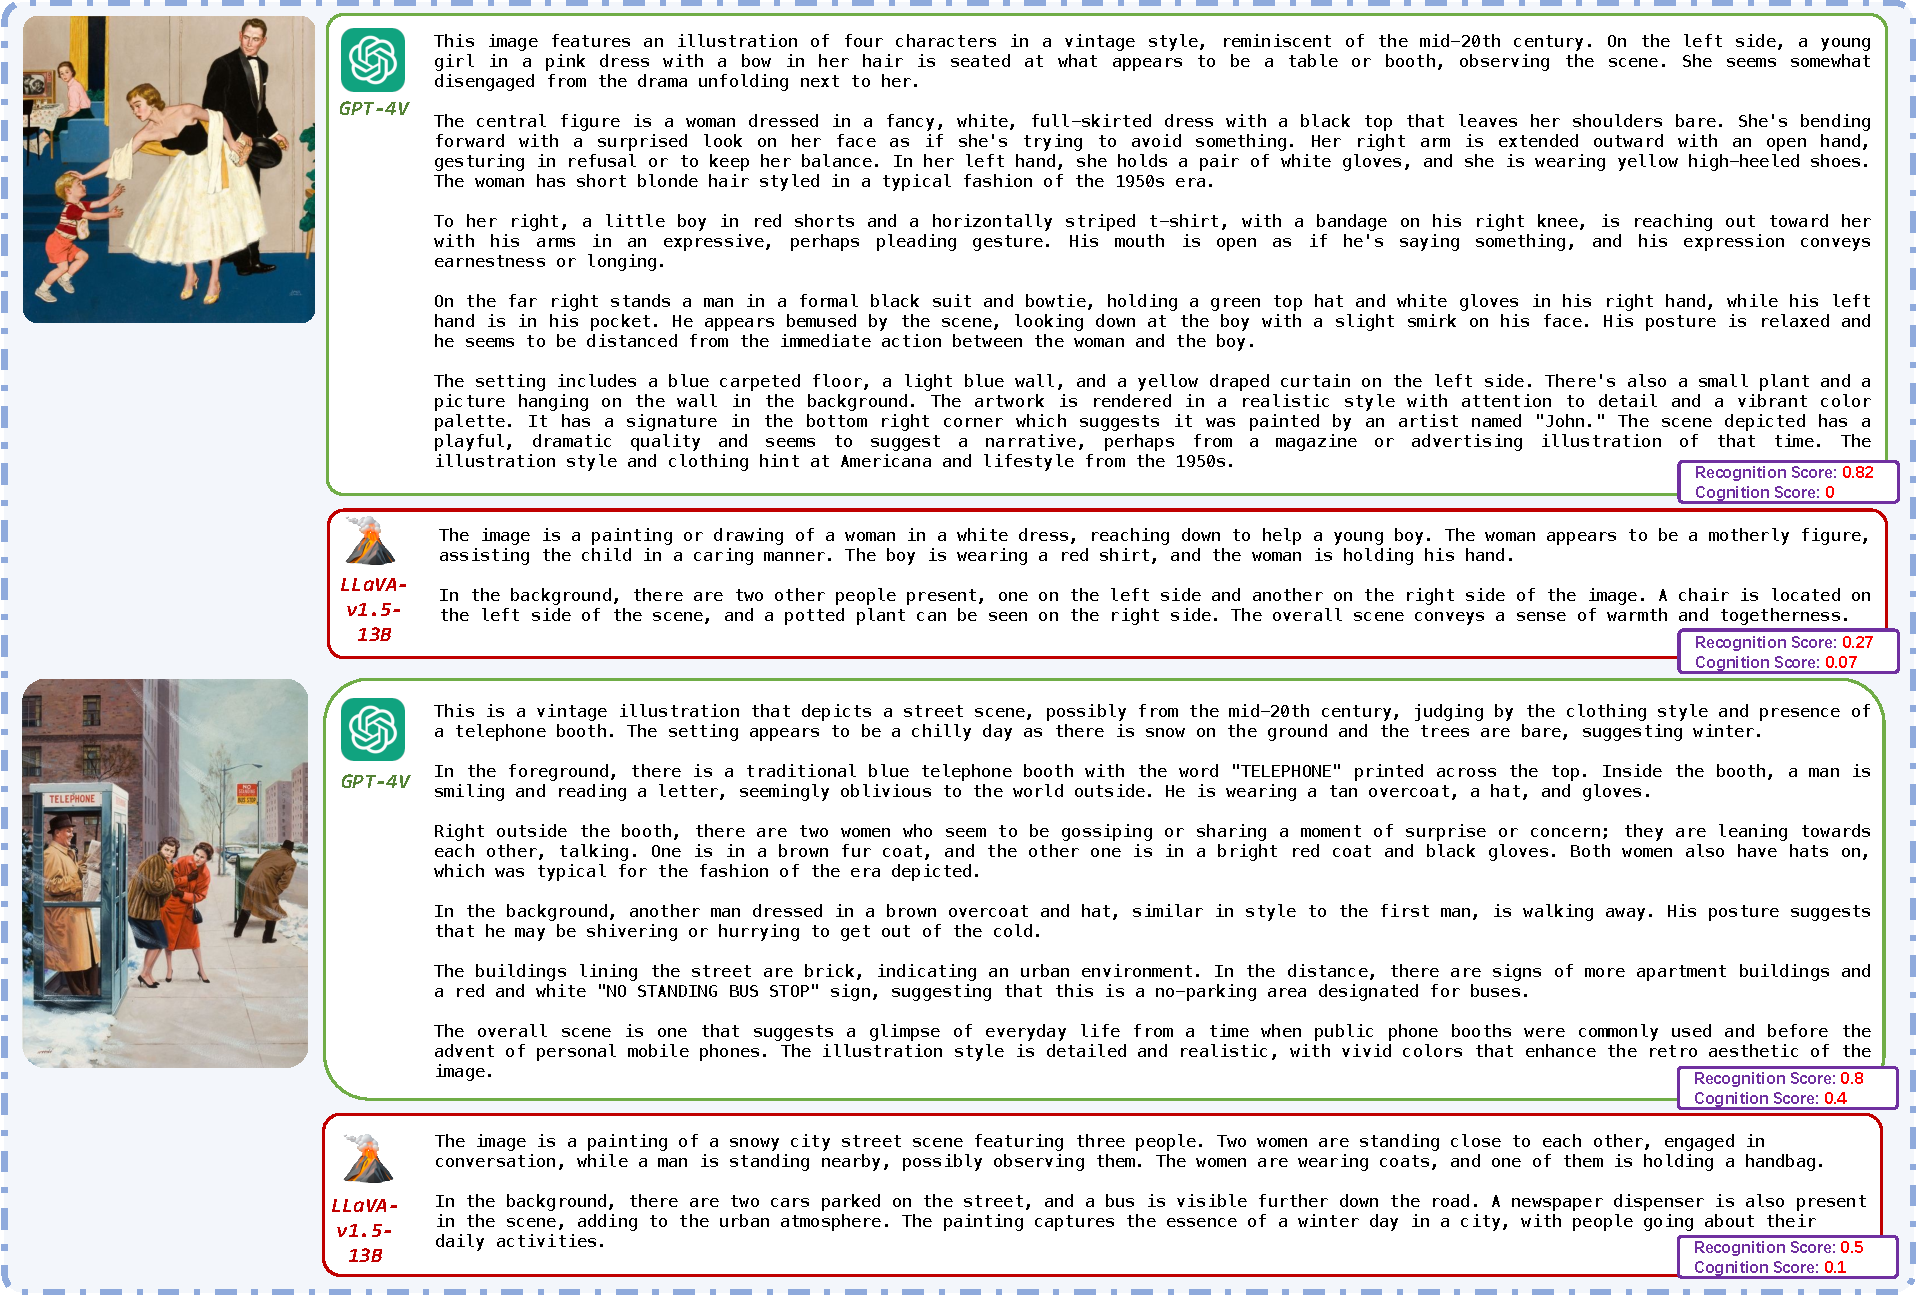
\includegraphics[width=0.95\textwidth]{figs/case2.pdf}
%     \caption{Case study of the Description task. GPT-4V and a representative open-source LVLM LLaVA-v1.5-13B is selected for analysis. \KZ{This pic takes
% too much space and should go into Appendix at least.}}
%     \label{fig:case}
% \end{figure*}

\begin{figure*}[th]
    \centering
    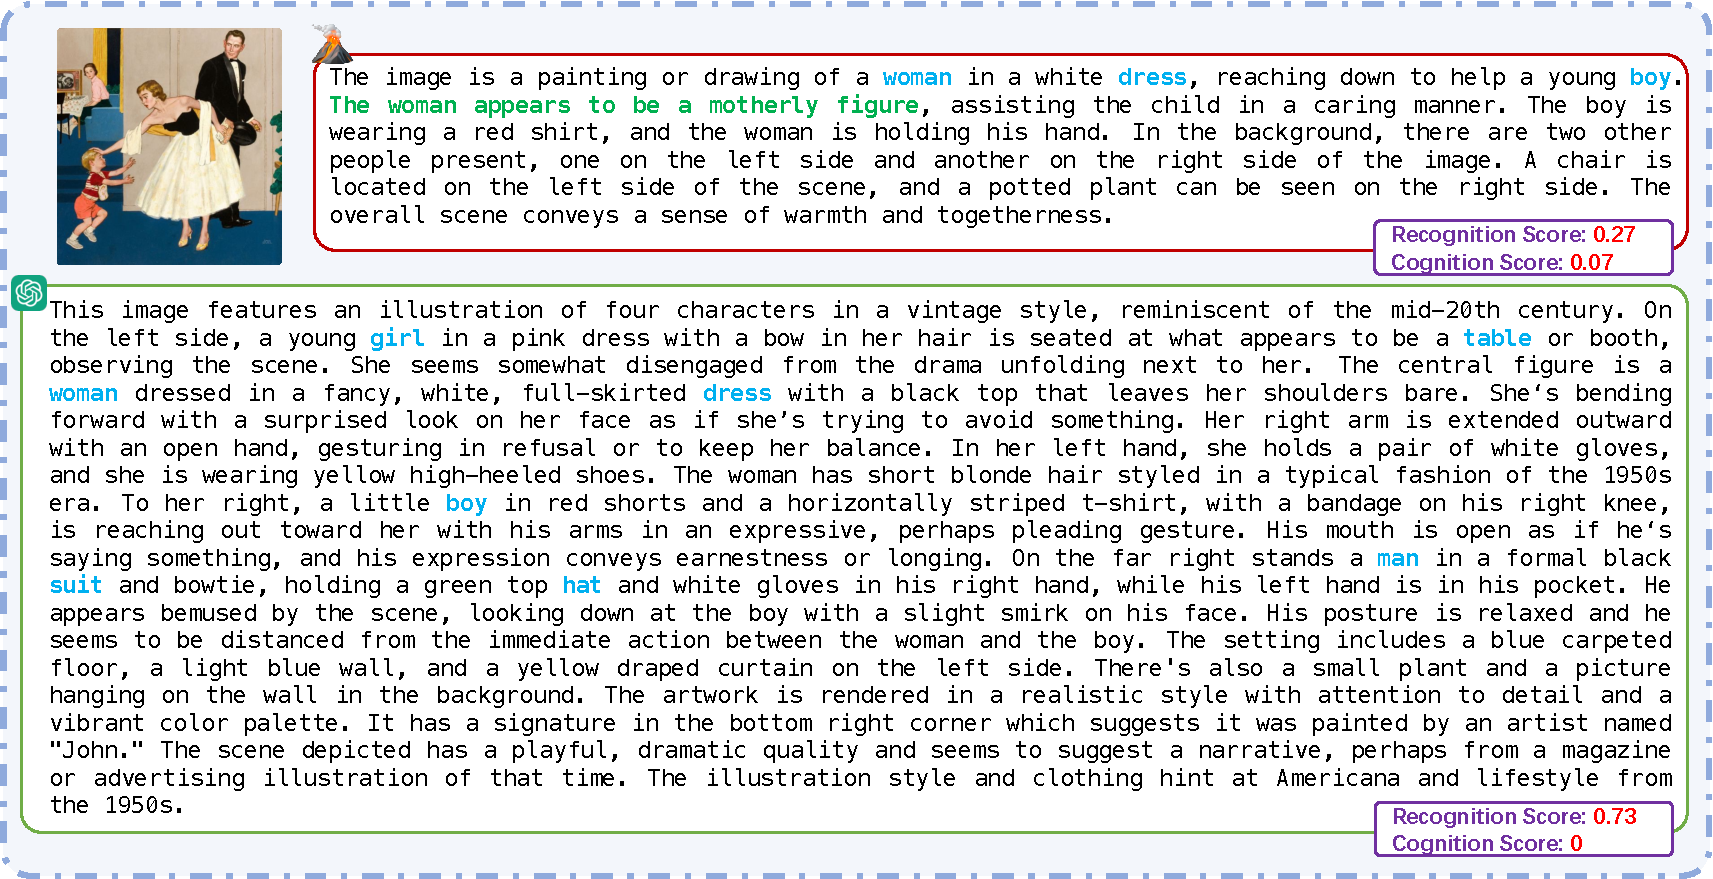
\includegraphics[width=0.9\textwidth]{figs/case_single3.pdf}
    \caption{Case study of the Description task. 
    A representative open-source LVLM LLaVA-v1.5-13B (red frame) and GPT-4V (green frame) are selected for analysis. 
    Recognized entities are marked in \textcolor{blue}{blue}, and CoRs are marked in \textcolor{c2}{green}.
    % \KZ{This pic takes too much space and should go into Appendix at least.}
    % \XJ{Removed one case.}
    }
    \label{fig:case}
\end{figure*}



\subsection{Results of VQA Task}

% % this table is calculated based on 95 pics
% \begin{table*}[h!]
%     \centering
%     \small
%     \setlength{\tabcolsep}{2.5pt} 
%     \begin{tabular}{lccccccccc}
%     \hline
%     \textbf{Model} & \thead{\textbf{Time} } & \thead{\textbf{Location} } & \thead{\textbf{Character} } &  \thead{\textbf{Character}\\ \textbf{Relationship} } & \thead{\textbf{Event} } & \thead{\textbf{Event} \\ \textbf{Relationship} } & \thead{\textbf{Mental} \\ \textbf{State} } & \thead{\textbf{Next}\\ \textbf{Moment} \\ \textbf{Event} } & \thead{\textbf{Overall} } \\ % \\ \textbf{Accuracy}
%     \hline
%     InstructBLIP-7B &  0.340 & 0.574 & 0.471 & 0.522 &  0.364 &  0.44 & 0.371 & 0.392 & 0.426 \\  % this is reults based on generation
%     Qwen-VL-Chat & 0.638 & 0.840 & 0.629 & 0.547 &  0.539 & 0.399 & 0.534 & 0.5 & 0.551 \\
%     LLaVA-V1.5-7B & 0.553 & 0.798 & 0.542 & 0.541 & 0.512 & 0.369 &  0.529 & 0.473 & 0.523 \\
%     LLaVA-V1.5-13B & 0.681 & 0.851 & 0.6 & 0.616 & 0.481 & 0.536 & 0.557 & 0.676 & 0.586 \\
%     % CogVLM & 0 & & & & & & & & \\
%     mPLUG-Owl-2 & 0.574 & 0.819 & 0.543 & 0.528 & 0.512 & 0.464 & 0.561 & 0.527 & 0.549 \\
%     ShareGPT4V-7B & 0.617 & 0.777 & 0.629 & 0.585 & 0.5 & 0.357 & 0.561 & 0.527 & 0.542 \\
%     ShareGPT4V-13B & 0.702  & 0.851 & 0.586 & 0.560 & 0.5  & 0.5 & 0.579 & 0.716 & 0.584 \\
%     % Monkey &  &  &  &  &  &  &  &  &  \\
%     GPT-4V & 0.723 & 0.883 & 0.786 & 0.686 & 0.678 & 0.649 & 0.706 & 0.716 & 0.709 \\
%     \hline
%     Human & 0.979 & 0.957 & 0.986 & 0.962 & 0.965 & 0.976 & 0.946 &  0.959 & 0.963 \\
%     \hline
%     \end{tabular}
%     \caption{\label{tab:cogvqa}
%     Model performance on VQA task. 
%     The accuracy of Human is calculated based on the responses of a healthy adult male.
%     % \KZ{Again, how ou got the human scores.}
%     }
% \end{table*}

% this table is calculated based on 95 pics
\begin{table*}[h!]
    \centering
    \small
    \setlength{\tabcolsep}{2.5pt} 
    \begin{tabular}{lccccccccc}
    \hline
    \textbf{Model} & \thead{\textbf{Time} } & \thead{\textbf{Location} } & \thead{\textbf{Character} } &  \thead{\textbf{Character}\\ \textbf{Relationship} } & \thead{\textbf{Event} } & \thead{\textbf{Event} \\ \textbf{Relationship} } & \thead{\textbf{Next}\\ \textbf{Moment} \\ \textbf{Event} } & \thead{\textbf{Mental} \\ \textbf{State} } & \thead{\textbf{Overall} } \\ % \\ \textbf{Accuracy}
    \hline
    InstructBLIP-7B &  0.34 & 0.57 & 0.47 & 0.52 &  0.36 &  0.44  & 0.39 & 0.37 & 0.43 \\  % this is reults based on generation
    Qwen-VL-Chat & 0.64 & 0.84 & 0.63 & 0.55 &  0.54 & 0.40  & 0.50 & 0.53 & 0.55 \\
    LLaVA-V1.5-7B & 0.55 & 0.80 & 0.54 & 0.54 & 0.51 & 0.37 & 0.47 &  0.53  & 0.52 \\
    LLaVA-V1.5-13B & 0.68 & 0.85 & 0.60 & 0.62 & 0.48 & 0.54 & 0.68 & 0.56 & 0.59 \\
    % CogVLM & 0 & & & & & & & & \\
    mPLUG-Owl-2 & 0.57 & 0.82 & 0.54 & 0.53 & 0.51 & 0.46  & 0.53 & 0.56 & 0.55 \\
    ShareGPT4V-7B & 0.62 & 0.78 & 0.63 & 0.59 & 0.50 & 0.36 & 0.53 & 0.56 & 0.54 \\
    ShareGPT4V-13B & 0.70  & 0.85 & 0.59 & 0.56 & 0.50  & 0.50  & 0.72 & 0.58 & 0.58 \\
    % Monkey &  &  &  &  &  &  &  &  &  \\
    GPT-4V & 0.72 & 0.88 & 0.79 & 0.69 & 0.68 & 0.65  & 0.72 & 0.71 & 0.71 \\
    \hline
    Human & 0.98 & 0.96 & 0.99 & 0.96 & 0.97 & 0.98 &  0.96 & 0.95 & 0.96 \\
    \hline
    \end{tabular}
    \caption{\label{tab:cogvqa}
    Model performance on VQA task. Each QA contains four options, with a chance rate of 25\%. 
    % The accuracy of Human is calculated based on the responses of a healthy adult male.
    % \KZ{Again, how ou got the human scores.}
    }
\end{table*}


Table \ref{tab:cogvqa} shows the performance of LVLMs on VQA task. 
Consistent with results in previous sections, GPT-4V achieves the best performance and there is a performance gap between GPT-4V and open-source models.
For open-source models, ShareGPT4V-13B and LLaVA-v1.5-13B achieves better performance than other LVLMs based on 7B LLMs, which shows the importance of LLM size to LVLMs.
As for LVLMs based on 7B LLMs, the performance of InstructBLIP is the worst and there is also a gap between InstructBLIP and other models. 
One possible reason is that it only finetunes the Q-former for instruction-tuning as Q-former has limited capacity compared with LLMs.
The performance of other models are similar.
Consistent with previous findings, reasoning about location is also the easiest for LVLMs and event-related reasoning are more difficult.
There is also a large gap between the performance of LVLMs and human beings.
Note that the accuracy of Human in Table \ref{tab:cogvqa} is calculated based on the responses of a healthy 24-year-old male with a Bachelor's degree.

% \begin{table*}
%     \centering
%     \small
%     \begin{tabular}{llllllllll}
%     \hline
%     \textbf{Model} & \thead{\textbf{Time} } & \thead{\textbf{Location} } & \thead{\textbf{Character} } &  \thead{\textbf{Character}\\ \textbf{Relationship} } & \thead{\textbf{Event} } & \thead{\textbf{Event} \\ \textbf{Relationship} } & \thead{\textbf{Mental} \\ \textbf{State} } & \thead{\textbf{Next}\\ \textbf{Moment} \\ \textbf{Event} } & \thead{\textbf{Overall} } \\ % \\ \textbf{Accuracy}
%     \hline
%     MiniGPT-4-7B  &  &  &  &  &  &  &  &  &  \\
%     InstructBLIP-7B & 0.434 & 0.523 & 0.55 & 0.559 & 0.425 & 0.437 & 0.342 & 0.436 & 0.451 \\
%     Otter & 0.301 & 0.606 & 0.362 & 0.441 & 0.306 & 0.272 & 0.404 & 0.333 & 0.376 \\
%     LLaVA-v1.5-7b & 0.641 & 0.844 & 0.6125 & 0.638 & 0.521 & 0.396 & 0.556 & 0.5 & 0.569 \\
%     LLaVA-v1.5-13b & 0.755 & 0.88 & 0.662 & 0.702 & 0.498 & 0.562 & 0.578 & 0.692 & 0.628 \\
%     % CogVLM & 0 & & & & & & & & \\
%     Qwen-VL & 0.735 & 0.908 & 0.725 & 0.670 & 0.582 & 0.485 & 0.6 & 0.577 & 0.633 \\
%     ShareGPT4V-7B & 0.660 & 0.817 & 0.7 & 0.691 & 0.510 & 0.379 & 0.564 & 0.577 & 0.584 \\
%     ShareGPT4V-13B & 0.755 & 0.872 & 0.675 & 0.654 & 0.517 & 0.515 & 0.618 & 0.744 & 0.629 \\
%     Monkey & 0.736 & 0.89 & 0.688 & 0.707 & 0.571 & 0.515 & 0.551 & 0.59 & 0.628 \\
%     GPT-4V & 0.774 & 0.917 & 0.8 & 0.723 & 0.686 & 0.669 & 0.729 & 0.769 & 0.737 \\
%     \hline
%     Human & 1.0 & 0.973 & 1.0 & 0.963 & 0.953 & 0.973 & 0.925 & 0.964 & 0.960 \\
%     \hline
%     \end{tabular}
%     \caption{\label{tab:cogqa}
%     CogVQA.
%     }
% \end{table*}

% % this table is calculated based on 94 pics
% \begin{table*}
%     \centering
%     \small
%     \begin{tabular}{lccccccccc}
%     \hline
%     \textbf{Model} & \thead{\textbf{Time} } & \thead{\textbf{Location} } & \thead{\textbf{Character} } &  \thead{\textbf{Character}\\ \textbf{Relationship} } & \thead{\textbf{Event} } & \thead{\textbf{Event} \\ \textbf{Relationship} } & \thead{\textbf{Mental} \\ \textbf{State} } & \thead{\textbf{Next}\\ \textbf{Moment} \\ \textbf{Event} } & \thead{\textbf{Overall} } \\ % \\ \textbf{Accuracy}
%     \hline
%     % InstructBLIP-7B & 0.362 & 0.376 & 0.471 & 0.437 & 0.396 & 0.406 & 0.309 & 0.397 & 0.388 \\     % this is results based on predict_class
%     InstructBLIP-7B & 0.34 & 0.570 & 0.471 & 0.519  & 0.360 & 0.436 & 0.378 & 0.397 & 0.426 \\  % this is reults based on generation
%     Qwen-VL-Chat & 0.638 & 0.839 & 0.629 & 0.544 & 0.541 & 0.388 & 0.544 & 0.507 & 0.552 \\
%     LLaVA-V1.5-7B & 0.553 & 0.796 & 0.543 & 0.538 & 0.510 & 0.364 & 0.539 & 0.466 & 0.523\\	
%     LLaVA-V1.5-13B & 0.681 & 0.849 & 0.6 & 0.614 & 0.478 & 0.533 & 0.567 & 0.671 & 0.586 \\
%     % CogVLM & 0 & & & & & & & & \\
%     mPLUG-Owl-2 & 0.574 & 0.817 & 0.543 & 0.525 & 0.510 & 0.461 & 0.571 & 0.534 & 0.55 \\
%     ShareGPT4V-7B & 0.617 & 0.774 & 0.629 & 0.582 & 0.498 & 0.358 & 0.567 & 0.521 & 0.542 \\
%     ShareGPT4V-13B & 0.702 & 0.849 & 0.586 & 0.557 & 0.498 & 0.497 & 0.590 & 0.712 & 0.584 \\
%     % Monkey &  &  &  &  &  &  &  &  &  \\
%     GPT-4V & 0.723 & 0.882 & 0.786 & 0.690 & 0.675 & 0.648 & 0.714 & 0.726 & 0.712 \\
%     % \hline
%     % Human &  &  &  &  &  &  &  &  &  \\
%     \hline
%     \end{tabular}
%     \caption{\label{tab:cogvqa}
%     Model performance on CogVQA task.
%     }
% \end{table*}




% \subsection{Effectiveness Analysis of GPT-based Cognition Evaluation of CogID}

% % Considering the interpretability issues 

% To prove the effectiveness of GPT-based evaluation, we manually annotated a subset by assigning 0/1 to CoRs of 20 images and use the subset to evaluate the performance of different evluation methods.

% Table \ref{tab:eval_metrics} shows the accuracy of different evaluation methods on the subset.
% It can be seen that GPT-4 achieves the best performance, which indicates that GPT-based evaluation is effective for evaluating the performance of LVLMs on CogID task.
% The implementation details of evaluation methods beyond ChatGPT and GPT-4 can be found in Appendix \ref{sec:eval_method}.




% % Details are shown in Appendix.
% % Besides, as the evaluation task is a fine-grained discriminative task, the interpretability problem of GPT can be alleviated to some extent.

% % before 20240204_95
% % \begin{table}
% %     \centering
% %     \small
% %     \begin{tabular}{lc}
% %     \hline
% %     \textbf{Model} & \textbf{Accuracy}\\ % \\ \textbf{Accuracy}
% %     \hline
% %     ROUGE  & 0.656 \\
% %     % ROUGE-paragraph & 0.567  \\
% %     BERTScore & 0.641 \\
% %     % BERTScore-paragraph & 0.620  \\
% %     BLEURT & 0.620 \\
% %     DeBERTa & 0.682 \\
% %     DocNLI  & 0.703 \\
% %     GPT-3.5 & 0.797 \\
% %     GPT-4 & 0.83 \\
% %     \hline
% %     \end{tabular}
% %     \caption{\label{tab:eval_metrics}
% %     Accuray of different evaluation methods on human evaluation.
% %     }
% % \end{table}

% % after 20240204_95
% \begin{table}
%     \centering
%     \small
%     \begin{tabular}{lc}
%     \hline
%     \textbf{Model} & \textbf{Accuracy}\\ % \\ \textbf{Accuracy}
%     \hline
%     ROUGE  & 0.656 \\
%     % ROUGE-paragraph & 0.567  \\
%     BERTScore & 0.635 \\
%     % BERTScore-paragraph & 0.620  \\
%     BLEURT & 0.620 \\
%     DeBERTa & 0.693 \\
%     DocNLI  & 0.714 \\
%     GPT-3.5 & 0.807 \\
%     GPT-4 & 0.849 \\
%     \hline
%     \end{tabular}
%     \caption{\label{tab:eval_metrics}
%     Accuray of different evaluation methods.
%     }
% \end{table}
